\documentclass[12pt]{amsart}
\usepackage{amsmath}
\usepackage{amssymb}
\usepackage[utf8]{inputenc}
\usepackage{tikz}
\usetikzlibrary{arrows,shapes,calc,snakes,shadows,positioning,cd}

\begin{document}

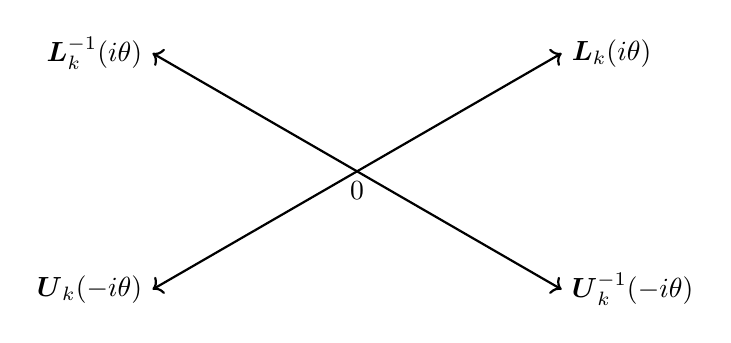
\begin{tikzpicture}[]

    %Contour lines
    \draw[thick] (0,0) -- (30:1.5cm);
    \draw[->,  thick] (30:1.5cm) -- (30:3cm) node[right=0cm] {$\boldsymbol{L}_k(i\theta)$};
    \draw[thick] (0,0) -- (150:1.5cm);
    \draw[->,  thick] (150:1.5cm) -- (150: 3cm) node[left=0cm] {$\boldsymbol{L}^{-1}_k(i\theta)$};
    \draw[thick] (0,0) -- (210: 1.5 cm);
    \draw[->,  thick] (210: 1.5cm) -- (210: 3cm) node[left=0cm] {$\boldsymbol{U}_{k}(-i\theta)$};
    \draw[thick] (0,0) -- (330: 1.5cm);
    \draw[->, thick] (330: 1.5 cm) -- (330: 3cm) node[right=0cm] {$\boldsymbol{U}_{k}^{-1}(-i\theta$)};
    \node at (0,-.25) {$0$};           
\end{tikzpicture}

\end{document}